\label{Chapter2}

\section{Μορφολογία και ανίχνευση ακμών}

Στο αυτό το κομμάτι της εργασίας, το ζητούμενο είναι να γίνει ανίχνευση των ακμών με την χρήση της τεχνικής Canny σε μία grayscale εικόνα. Στην συνέχεια, πρέπει να προστεθεί και να παρατηρηθούν οι αλλαγές.

\subsection{Τεχνική Canny}

H τεχνική ανίχνευση ακμών Canny είναι ένας διάσημος αλγόριθμος ανίχνευσης ακμών. Για να ολοκληρωθεί και να βρει τις ακμές περνάει από μερικά στάδια. Στην Python, παράγεται έτοιμο. Ο κώδικας είναι ο εξής:

\begin{minted}{py}
def apply_edges(image, t_lower=100, t_upper=200, aperture_size=5, L2Gradient=True) -> any:
  return cv2.Canny(
    image, t_lower, t_upper,
    apertureSize=aperture_size, L2gradient=L2Gradient
  )
\end{minted}

Η φωτογραφία που επιλέχτηκε για να γίνει η ανίχνευση των ακμών βρίσκετε στο Σχήμα~\ref{fig:guitar_god}, ενώ τα αποτελέσματα του αλγορίθμου στο Σχήμα~\ref{fig:original}.

\begin{figure}[H]
  \centering
  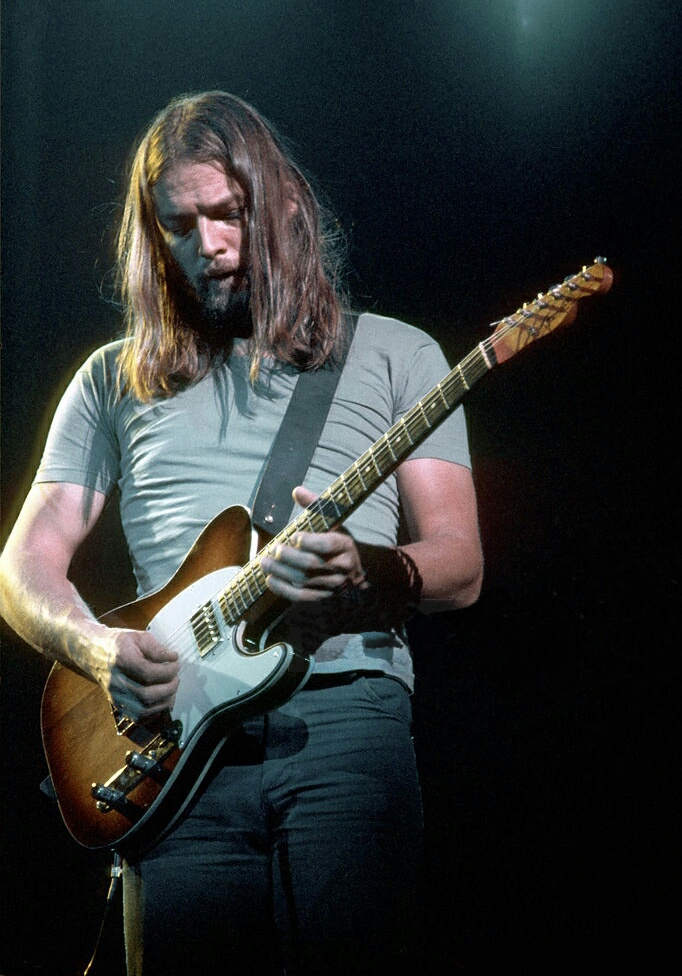
\includegraphics[width=100mm]{Figures/david_gilmour}
  \caption[David Gilmour]{Ο David Gilmour, γνωστός για την συμμετοχή του στο συγκρότημα Pink Floyd και ως τρομερός μουσικός}
  \label{fig:guitar_god}
\end{figure}

\begin{figure}[H]
  \centering
  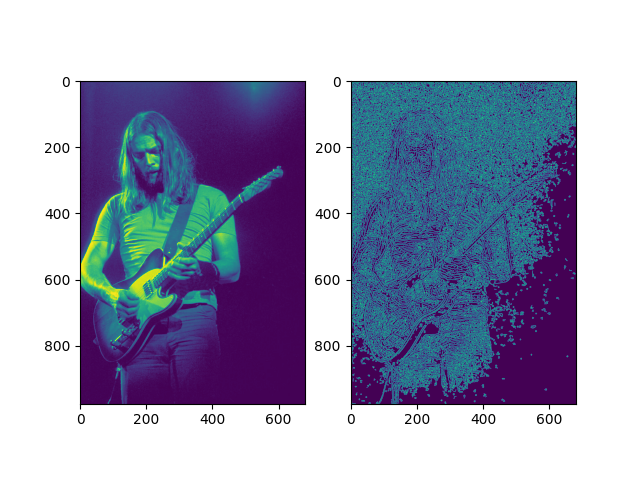
\includegraphics[width=100mm]{Figures/Original}
  \caption[Η σύγκριση του Original με την τεχνική canning]{Η σύγκριση του Original με την τεχνική canning. Να παρατηρηθεί ότι ο ίδιος φαίνεται ελάχιστα και πιάνει πολύ background noise ο αλγόριθμος}
  \label{fig:original}
\end{figure}

\subsection{Γκαουσιανός θόρυβος}

Εφαρμογή αλγορίθμου για προσθήκη Γκαουσιανού θορύβου στην εικόνα.

\begin{minted}{py}
def add_noise_and_remove_it(image) -> any:
  gaussian_noise = np.random.normal(0, 1, image.size)
  gaussian_noise = gaussian_noise.reshape(image.shape[0], image.shape[1]).astype('uint8')
  noise = cv2.add(image, gaussian_noise)
  return cv2.medianBlur(noise, 5)
\end{minted}

Στο Σχήμα~\ref{fig:restored}, μπορεί να βγει το συμπέρασμα ότι προσθέτοντας θόρυβο στην εικόνα, μπορεί να βοηθήσει την τεχνική Canny για να εντοπίσει πιο σωστά τις ακμές της εικόνας.

\begin{figure}[H]
  \centering
  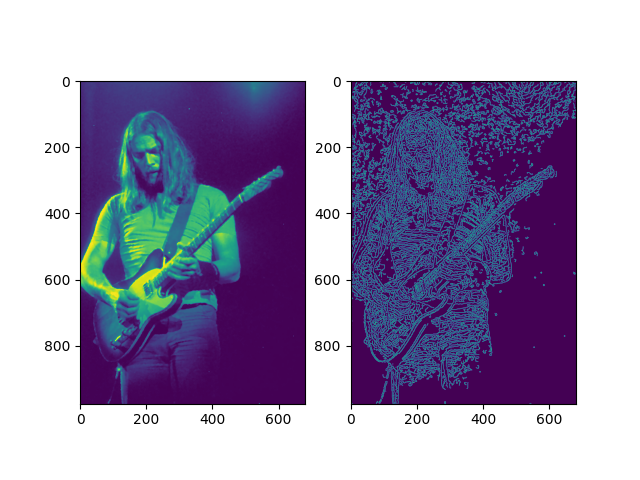
\includegraphics[width=100mm]{Figures/Restored}
  \caption[Η σύγκριση της επαναφοράς της εικόνας με την τεχνική canning]{Η σύγκριση της επαναφοράς της εικόνας με την τεχνική canning. Να παρατηρηθεί ότι ο ίδιος φαίνεται πολύ καλύτερα και μπορεί να παρατηρηθεί η μορφή του γνωστού κιθαρίστα}
  \label{fig:restored}
\end{figure}

\subsection{Συνδυασμός μορφολογίας με σύγκριση ακμών}

Μορφολογία στην επεξεργασία εικόνας είναι το πως αναπαριστάτε η κάθε φιγούρα μέσα στην εικόνα. Υπάρχουν δύο μορφολογικοί τελεστές που χρησιμοποιήθηκαν σε αυτή την εργασία είναι ο erosion και ο dilation.

\subsubsection{Μορφολογικός Τελεστής Erosion}

\begin{equation}
  Α \ominus Β = \{ z | (Β)_z \subseteq Α \}
\end{equation}

\begin{figure}[H]
  \centering
  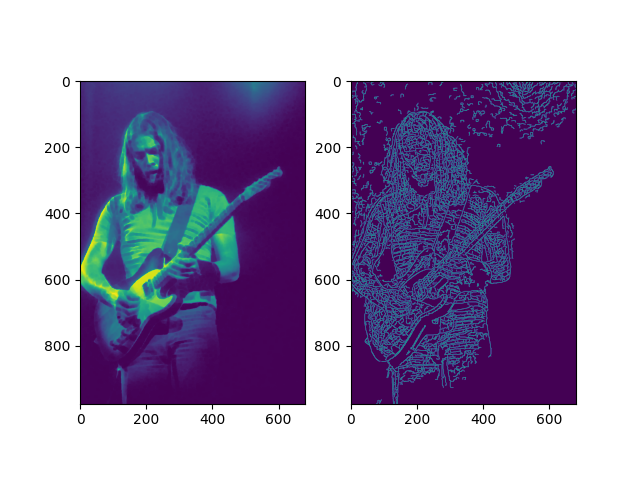
\includegraphics[width=100mm]{Figures/Erosion}
  \caption[Η σύγκριση της επαναφοράς της εικόνας αφού έχει περαστεί απο erosion με την τεχνική canning]{Η σύγκριση της επαναφοράς της εικόνας αφού έχει περαστεί από erosion με την τεχνική canning. Η μορφή του κιθαρίστα είναι ακόμα πιο καθαρή από πριν, βεβαία περνάει και λίγο από το background noise μέσα στις ακμές του}
  \label{fig:erosion}
\end{figure}

\newpage
\subsubsection{Μορφολογικός Τελεστής Dilation}

\begin{equation}
  Α \oplus Β = \{ z | (\hat{Β})_z \cap Α \}
\end{equation}

\begin{figure}[H]
  \centering
  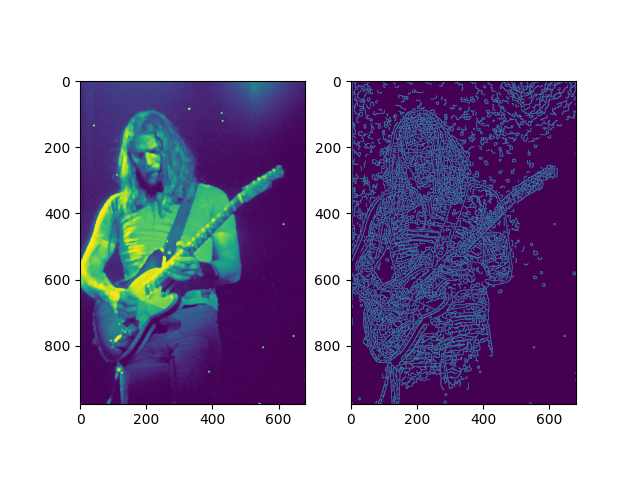
\includegraphics[width=100mm]{Figures/Dilation}
  \caption[Η σύγκριση της επαναφοράς της εικόνας αφού έχει περαστεί απο dilation με την τεχνική canning]{Η σύγκριση της επαναφοράς της εικόνας αφού έχει περαστεί από dilation με την τεχνική canning. Η μορφή του κιθαρίστα είναι αρκετά ίδια με το erosion, με την διαφορά ότι έχει παραπάνω θόρυβο}
  \label{fig:dilation}
\end{figure}

\subsection{Σύγκριμα αποτελεσμάτων με την χρήση αλγορίθμων}

Για το πόσο καλά αποτελέσματα παράγει ο αλγόριθμος, θα ακολουθούν διάφορες τεχνικές. Για να γίνει οποιαδήποτε σύγκριση όμως χρειάζεται να γίνει μετατροπή των εικόνων σε ιστογράμματα για να είναι πιο επεξεργάσιμοι από τους καθημερινούς μοντέρνους υπολογιστές. Ο αλγόριθμος δοκιμάστηκε σε σταθερό υπολογιστή με Ryzen 5 2600 και 8 GB ram και είχε ελάχιστη καθυστέρηση.

\subsubsection{Ευκλειδική Διαφορά}

Η πρώτη διαφορά που θα μελετηθεί είναι η Ευκλειδική. Ο αλγόριθμος είναι ο εξής:

\begin{minted}{py}
euclidean = 0
i = 0
while i < len(histogram_original) and i < len(histogram_edges):
  euclidean += (histogram_original[i] - histogram_edges[i]) ** 2
  i += 1
\end{minted}

\begin{table}[H]
  \centering
	\begin{tabular}{ | p{8cm} | p{8cm} | }
		\hline
		\textbf{Όνομα εικόνας} & \textbf{Αποτέλεσμα Ευκλειδικής Διαφοράς} \\
    \hline
    Original εικόνα & 1.3595214842916974 \\
    \hline
    Restored εικόνα & 1.4140797849329154 \\
    \hline
    Restored εικόνα με Erosion & 1.4136366487406054 \\
    \hline
    Restored εικόνα με Delation & 1.4135856679087746 \\
    \hline
	\end{tabular}
  \caption{Αποτελέσματα Ευκλειδικής διαφοράς}
  \label{tab:euclidean}
\end{table}

\newpage
\subsubsection{$ X^2 $ Διαφορά}

Η δεύτερη διαφορά είναι η $ X ^ 2 $ διαφορά. Δίνετε έτοιμο από το cv2.

\begin{table}[H]
  \centering
	\begin{tabular}{ | p{8cm} | p{8cm} | }
		\hline
		\textbf{Όνομα εικόνας} & \textbf{Αποτέλεσμα $ X^2 $ Διαφοράς} \\
    \hline
    Original εικόνα & 55.54426650712792 \\
    \hline
    Restored εικόνα & 9917.798371611698 \\
    \hline
    Restored εικόνα με Erosion & 1213.5299873964364 \\
    \hline
    Restored εικόνα με Delation & 7.813439429146478 \\
    \hline
	\end{tabular}
  \caption{Αποτελέσματα $ X^2 $ διαφοράς}
  \label{tab:chi_squared}
\end{table}

\subsubsection{Bhattacharyya Διαφορά}

Η τρίτη διαφορά είναι η Bhattacharyya διαφορά. Δίνετε έτοιμο από το cv2.

\begin{table}[H]
  \centering
	\begin{tabular}{ | p{8cm} | p{8cm} | }
		\hline
		\textbf{Όνομα εικόνας} & \textbf{Αποτέλεσμα Bhattacharyya Διαφοράς} \\
    \hline
    Original εικόνα & 0.9437122663789763 \\
    \hline
    Restored εικόνα & 0.9962561700845681 \\
    \hline
    Restored εικόνα με Erosion & 0.993916915962169 \\
    \hline
    Restored εικόνα με Delation & 0.9944792139506231 \\
    \hline
	\end{tabular}
  \caption{Αποτελέσματα Bhattacharyya διαφοράς}
  \label{tab:bhattacharyya}
\end{table}

\subsubsection{Correlation Διαφορά}

Η τέταρτη διαφορά είναι η correlation διαφορά. Δίνετε έτοιμο από το cv2.

\begin{table}[H]
  \centering
	\begin{tabular}{ | p{8cm} | p{8cm} | }
		\hline
		\textbf{Όνομα εικόνας} & \textbf{Αποτέλεσμα Correlation Διαφοράς} \\
    \hline
    Original εικόνα & 0.05002108348803092 \\
    \hline
    Restored εικόνα & -0.028392138047218348 \\
    \hline
    Restored εικόνα με Erosion & -0.022036753262860056 \\
    \hline
    Restored εικόνα με Delation & -0.030544818302308076 \\
    \hline
	\end{tabular}
  \caption{Αποτελέσματα Correlation διαφοράς}
  \label{tab:correlation}
\end{table}

\subsubsection{Intersection Διαφορά}

Η τελευταία διαφορά είναι η Intersection διαφορά. Δίνετε έτοιμο από το cv2.

\begin{table}[H]
  \centering
	\begin{tabular}{ | p{8cm} | p{8cm} | }
		\hline
		\textbf{Όνομα εικόνας} & \textbf{Αποτέλεσμα Intersection Διαφοράς} \\
    \hline
    Original εικόνα & 0.08144057751633227 \\
    \hline
    Restored εικόνα & 0.0007671799830859527 \\
    \hline
    Restored εικόνα με Erosion & 0.0008191215456463397 \\
    \hline
    Restored εικόνα με Delation & 0.008301599882543087 \\
    \hline
	\end{tabular}
  \caption{Αποτελέσματα Intersection διαφοράς}
  \label{tab:intersection}
\end{table}
